
\documentclass[12pt]{article}

\title{The Public Factor Exposure of Private Equity}

\author{
	Christian Tausch  \\
	AssetMetrix GmbH  \\
	Theresienh\"{o}he 13, D-80339 Munich \\
	christian.tausch@quant-unit.com \\
	\and 
	Marcus Pietz  \\
	AssetMetrix GmbH  \\
	Theresienh\"{o}he 13, D-80339 Munich \\
	marcus.pietz@asset-metrix.com \\
	}

\date{\today}



% Packages
\usepackage{amssymb}
\usepackage{amsmath}
\usepackage{natbib}
\usepackage{graphics}
% use smaller margins
\usepackage[margin=1.1in]{geometry} % 1.25in
\usepackage[margin=1.1cm]{caption}
% use double spacing
\usepackage{setspace}
\usepackage{amsthm}
\usepackage{url}
\usepackage[outdir=./]{epstopdf}
\usepackage{booktabs}
\usepackage{float}

\newtheorem{prop}{Proposition}
\newtheorem{assume}{Assumption}


% logo
\usepackage{fancyhdr}
\usepackage{graphicx }

\iffalse
%\addtolength{\headheight}{1cm} % make more space for the header
\pagestyle{fancyplain} % use fancy for all pages except chapter start
\lhead{
\includegraphics[height=0.6cm]{logo/quantunitcom}} % left logo
\rhead{
\includegraphics[height=0.6cm]{logo/AssetMetrixLogo2019schwarz}} % right logo
%\renewcommand{\headrulewidth}{0pt} % remove rule below header
\renewcommand{\chaptermark}[1]{ \markboth{#1}{} }
\renewcommand{\sectionmark}[1]{ \markright{#1}{} }
\fi


\begin{document}

\maketitle


\section*{Keywords}
 Public factor exposure, Private equity, Stochastic discount factor, Model combination, Factor investing, Ensemble learning


\section*{Acknowledgements}
We thank Nicolas D\"{u}tsch and Philipp Abel for valuable feedback and helpful comments that greatly improved the paper.


\section*{Declaration of interest}
The authors report no conflict of interest. 
The authors alone are responsible for the content and writing of the paper.


\newpage
%\doublespacing

\begin{center} 
\section*{The Public Factor Exposure of Private Equity}
\end{center}


\abstract{
	We propose Stochastic Discount Factor (SDF) model combination to determine the public factor exposure of private equity.
	First, we describe our theoretical motivation to favor model combination over model selection.
	This entails that we apply simple coefficient averaging to obtain multivariate SDF models that mimic the factor exposure of all major private capital fund types.
	The empirical results indicate that the replication strategies for the most conventional private equity fund types slightly outperform the (unlevered) MSCI World index in our sample period.
	Finally, we outline how to employ these factor models for integrated public and private risk management. 
}


\section{Introduction}
\label{sec:factor_investing}

Factor investing is currently popular in public markets as it helps investors to identify underlying return drivers.
Describing a portfolio's public factor exposure corresponds to understanding both its (i) realized returns and (ii) forward-looking risk and return expectations.
Realistic factor decompositions offer nuanced insights also for private market investors, assuming there exist common components that drive public and private returns.
From this viewpoint, factor analysis translates private equity returns to traded return components with main applications in public market equivalent benchmarking and holistic risk management.

Generally, more sophisticated methods are required to estimate factor models for private (in comparison to public) asset classes as private returns are not directly observable on liquid secondary markets.
However, the challenge of identifying the 'best' factor model is the same as in public markets.
There are first attempts to select or create public indices that shall replicate private equity (PE) returns.
Here, we can distinguish between (i) factor- and (ii) holding-based approaches.
\cite{P14} benchmarks buyout funds by several factor indices.
More subtle factor-based methods are mainly established in the hedge fund replication literature \citep{TV08,W14}.
To avoid overfitting, \cite{OST17} propose to combine multiple factor models for passive hedge fund replication.
Holding-based approaches to mimic the PE investment style are proposed by \cite{LSSL16}, \cite{S17}, \cite{MS19}, and \cite{PP19}.
This paper pursues a factor-based solution that employs publicly traded indices and does not require deal-level information on PE funds.
In contrast to the factor-based ansatz of \cite{P14}, we base our approach on SDF models that are actually estimated on PE fund-level data rather than comparing several ad-hoc choices for potentially suitable indices.

This article aims at a data-science-driven solution to describe PE returns.
Concretely, we propose SDF model combination as a straightforward method to obtain 'strong' public factor models that explain private equity returns.
Here, we provisionally define the term 'strong' versus 'weak' model in analogy to the boosting literature \citep{S90}.
A 'strong' model shall exhibit small (error term) bias and variance, whereas a 'weak' model displays high bias and variance.
Just the 'true' or 'best' or 'optimal' model obtains an error term of precisely zero.
Figure \ref{fig:how} illustrates our general ensemble-based approach to derive the public factor exposure of private equity \citep{B12}.

The paper is structured as follows.
Section \ref{sec:semiparametric_setting} introduces the method's underlying semiparametric setting.
Section \ref{sec:model_selection} explains why model selection is problematic.
Section \ref{sec:model_combination} argues that model combination is more promising.
Section \ref{sec:applications} presents two examples of how to apply our combined SDF models in the benchmarking and risk context.
Section \ref{sec:conclusion} concludes.

\begin{figure}[ht]
	\centering
	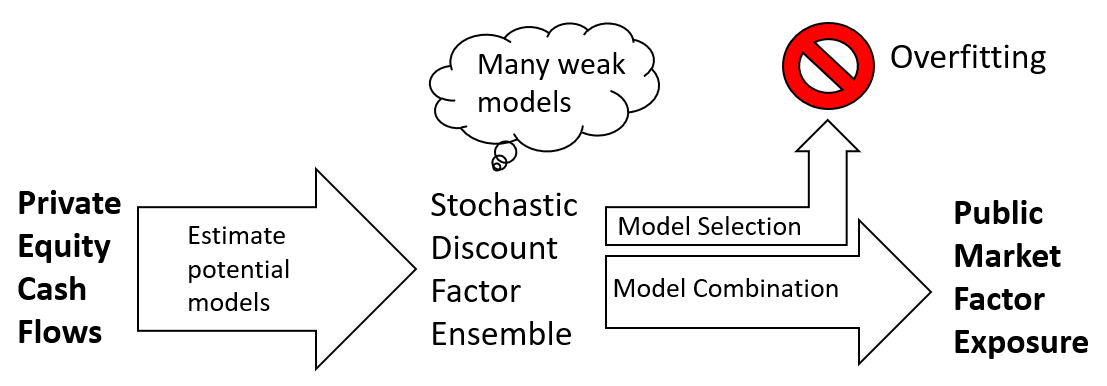
\includegraphics[width=14cm]{FlowChart/FC4}
	\caption{How to translate private equity cash flows to public market factors?}
	\label{fig:how}
\end{figure}

\section{Semiparametric setting}
\label{sec:semiparametric_setting}

Stochastic Discount Factors (SDFs) are econometric models to price a given cash flow stream \citep{HR87}.
They are usually estimated by semiparametric approaches that go without a parametric model for the error term \citep{F19}.
In our case, the cash flows stream under consideration is generated by $i=1,2,\dots,n$ private equity funds (or portfolios).
SDFs can be applied in net present value calculations for realized cash flow paths
\begin{equation}
\label{eq:pricing_error}
P_{\tau, t, i} =
\sum_{t=1}^{T}\ \Psi_{\tau, t}\ {CF}_{t, i}
\end{equation}
with price (or pricing error) $P$, SDF functional $\Psi$, and cash flow stream $CF$. 
If the 'true' SDF model is applied, the expected price $\mathbb{E}[P]=0$. 
Thus the functional form and explanatory variables used in the 'true' SDF explain or describe the risk and return properties of the cash flows. 
Further, if we have an appropriate SDF for a given private equity fund type, we can apply it in a simple net present value calculation (as in the formula above) to assess the outperformance of a specific private equity fund. 
A positive/negative net present value indicates an out/under-performance compared to other PE funds.
To discount a time $t$ cash flow to time $\tau$, we use the simple linear multi-period SDF model
\begin{equation}
\label{eq:linear_sdf}
\Psi_{\tau,t} =
\prod_{h=0}^{t}\ \left(1+ \alpha + r_{h} + \sum_j\ \beta_j\ F_{j,h} \right)^{-1}
\prod_{h=0}^{\tau}\ \left(1 + \alpha + r_{h} + \sum_j\ \beta_j\ F_{j,h} \right)
\end{equation}
with usually $\alpha=0$, risk-free rate $r$, zero-net-investment factor return $F$, and factor coefficient $\beta$ that has to be estimated from data. 
Consequently, the expected multi-period return for a given asset is modeled by
\[
E \left[R_{\tau,t} \right] = \frac{1}{\Psi_{\tau,t}} + \epsilon_{\tau,t}
\]
where the period-specific error term $\epsilon_{\tau,t}$ has zero expectation $E[\epsilon_{\tau,t}]=0$.

As commonly seen in the asset pricing literature, we estimate SDF model coefficients by semiparametric approaches that require no distributional assumption for $\epsilon_{\tau,t}$.
This means we select $\alpha$ and $\beta$ values that yield average pricing errors close to zero. 
Here the typical loss function choices are quadratic forms like in Generalized Method of Moments (GMM) or a quadratic or least absolute deviance loss function $L()$
\begin{equation}
\label{eq:elastic_net}
\hat{\theta } = \
\arg \min_{\theta} L \left( P ; \theta, \gamma \right)
\end{equation}
where $\theta=(\alpha,\beta)$ and $\gamma$ denotes the vector of potential hyperparameters like data cutoff dates or weighting methods.
More details on the semiparametric estimation framework can be found in \cite{DLP12} and \cite{T20}.


\section{So many weak SDF model candidates}
\label{sec:model_selection}

Under the semiparametric setting described in section \ref{sec:semiparametric_setting}, we likely obtain many weak model candidates with no clear winner among them\footnote{This situation is comparable to the exuberant factor model zoo exclaimed for public equity by e.g., \cite{C11,FGX20}. Also, the vast public market literature is indecisive which factors best explain their assets' returns.}.
In this section, we explain in greater detail why we expect to be confronted with so (i) many but (ii) weak SDF models.
Moreover, we discuss why it is challenging to select the single 'best' model from an extensive collection of homogeneous competitors (that all use the same SDF model specified in equation \ref{eq:linear_sdf}).

\paragraph{Why so many models?}

\begin{itemize}
	\item There exists a great variety of different public return factor candidates that might be also relevant for private equity. It is not even clear which factors 'best' explain public equity returns, cf. references in \cite{KN20}. 
	\item We can choose from many feasible semiparametric estimators, loss functions, or ancillary machine learning methods, cf. \cite{GKX20} for a public market overview.
	Additionally, there are discretionary choices for regularization- or other hyper-parameters.
	Further, bootstrapping and other resampling-based techniques may be helpful but likewise dramatically increase the number of model candidates.
	\item In contrast to common public databases available for public equity, the private equity literature has to draw on various private - often proprietary - data sources. When estimating the same model on different datasets, the coefficient estimates will differ. Unclear data cutoff dates or horizons exacerbate this issue.
\end{itemize}

\paragraph{Why so weak models?}

\begin{itemize}
	\item Private equity data is notoriously sparse as the first PE funds were established in the 1970s or 80s. Moreover, it is currently (almost) impossible to collect data on all funds from a given vintage. These issues render finite [infinite] sample inference more [less] reliable.
	\item For fund-level data, the dependency issue introduced by overlapping fund cash flows further reduces the number of independent observations.
	\item In private equity, limited sample sizes typically allow the inclusion of just 1-2 factors in a SDF model; even many two factor models appear to be statistically insignificant (weak models); models with more covariates almost surely overfit (invalid models).
\end{itemize}

\paragraph{Why model selection is difficult?}

\begin{itemize}
	\item Model uncertainty is particularly high for weak models, as we cannot be sure which single model performs best when we test several competing models/factors.
	\item As there are many model candidates but limited data, data snooping may be a general problem \citep{W00}. 
	\item Correct inference post model selection is essential but known to be challenging \citep{BLP19}. This means classical statistical inference results just apply for testing a single model. When we want to compare several model candidates, the application of these basic statistical methods yields invalid inference results.
\end{itemize}



\section{And the jury selects... a strong combination}
\label{sec:model_combination}

A powerful alternative to model selection is model combination.
Generally, Bayesian and frequentist model averaging is a well-studied field in classical statistics \citep{H14,M15}.
Similarly, ensemble learning, a prominent subfield of machine learning, builds on the notion to form a strong learner by combining many weak learners \citep{B12}.
In more applied settings, predictive forecast combination often helps to increase forecast precision \citep{HL10}.
In a public market setting, \cite{RSZ10} forecast the public equity premium by combining 15 univariate OLS regressions of different macroeconomic predictors.
Probably most closely related to our case, \cite{OST17} advertise model combination for passive hedge fund replication.


\subsection{Model averaging}
\label{sec:model_averaging}

As we potentially want to exclude invalid models from combination, the set of valid models is defined as the $M^*$ models with the smallest absolute pricing error $M^*=\{m \in M: P^{(m)} \leq Q(\gamma;P) \}$ where $Q$ is the pricing error quantile function and $\gamma = \frac{M^*}{M}$.
Here, $M$ is the number of all valid and invalid SDF models.
Generally, we can also apply more sophisitcated (but also more time-consuming) cross-validation procedures to distinguish between valid and invalid models \citep{AC10}.
The quite different alternative is to assume that all SDF models estimated by the researcher are valid, i.e., $M^*=M$ with $\gamma=1$.
Finally, the weighted pricing error obtained by SDF model averaging is defined as
\begin{equation}
\label{eq:model_averaging}
\epsilon_{\tau, i}^{(M^*)} = 
\sum_{m=1}^{M^*} \  
w_m \
\sum_{t=1}^{T} \
\Psi_{\tau,t}^{(m)}\ 
{CF}_{t, i}
\end{equation}
with model weight $w_m \geq 0$ and all weights sum to one $\sum_m^{M^*}\ w_m=1$. 
If a similar predictive performance for all valid models can be assumed, equal weighting $w=(M^*)^{-1}$ is advised\footnote{The forecast combination puzzle states that simple equal-weighting practically often performs better than more complex (theoretically optimal) combination schemes \citep{SW09,CMVW16,QRCY19}.}. 
Otherwise, we shall overweight more predictive models with smaller pricing errors, e.g., the weight may be proportional to the inverse of the absolute pricing error $\left(\left|P_i\right|\right)^{-1}$.

\subsection{Coefficient averaging}
\label{sec:coef_averaging}

The general model combination approach defined by equation \ref{eq:model_averaging} allows the aggregation of structurally distinct SDF models.
If we always employ the same linear SDF as defined in equation \ref{eq:linear_sdf} (i.e., an attainable portfolio return, investable trading strategy), model combination can be interpreted as a diversification strategy.
The idea is to invest in several promising strategies instead of going all-in with one 'optimal' trading strategy.
Using always the same linear SDF model enables the following coefficient averaging formula, which only approximates the diversified pricing error from equation \ref{eq:model_averaging} (the better when the factor returns - thus return horizons - are small).
\begin{equation}
\label{eq:coef_averaging}
\beta_j^{(M^*)}\ =\ \sum_{m=1}^{M^*}\ w_m \ \beta_{j,m}
\end{equation}
The idea here is that one multivariate model that includes all traded factors can be better perceived and interpreted as an ensemble of $M^*$ heterogeneous one- or two-factor models.

Finally, with the $\beta_j^{(M^*)}$ coefficient estimated, we can focus on the $\alpha$ term in equation \ref{eq:linear_sdf}.
To quantify the public market out/underperformance, we can apply the Excess-IRR method described by \cite{PG09}, which estimates the $\alpha$ term by setting the pricing error to precisely zero for each $i$
\[
\hat{\alpha}_i = \arg \min_{\alpha_i} \left| P_{\tau, i}^{(M^*)}  \right|
\]
Alternatively, we can directly calculate the Internal Rate of Return (IRR) associated with the SDF discounted cash flows (with $\alpha=0$ in equation \ref{eq:linear_sdf}), which corresponds to the direct-alpha method described by \cite{GGS14}.
In both cases, we estimate the constant out/underperformance term for the $i$th portfolio after adjusting for systematic risk factors.

\section{Applications}
\label{sec:applications}

\subsection{Factor exposure by fund type}
\label{sec:factor_exposure}

% latex table generated in R 3.4.2 by xtable 1.8-4 package
% Wed Jul  1 13:54:55 2020
\begin{table}[ht]
	\centering
	\begin{tabular}{l@{\hskip 0.3in}l@{\hskip 0.2in}l@{\hskip 0.2in}l@{\hskip 0.2in}l@{\hskip 0.2in}l@{\hskip 0.1in}}
		Type & MKT-RF & HML & SMB & HDY-MKT & QLT-MKT \\ 
		\hline
		\hline
		BO & 1.33 (0.15) & -0.15 (0.12) & 0.2 (0.03) & 0.3 (0.1) & 0.21 (0.05) \\ 
		DD & 0.96 (0.09) & -0.11 (0.04) & 0.21 (0.01) & 0.14 (0.1) & 0.16 (0.05) \\ 
		%FOF & 1.22 (0.23) & -0.43 (0.09) & -0.24 (0.05) & -0.54 (0.09) & -0.01 (0.04) \\ 
		INF & 0.71 (0.22) & -0.37 (0.06) & -0.33 (0.13) & -0.47 (0.35) & 0.36 (0.11) \\ 
		MEZZ & 1.08 (0.13) & 0.06 (0.1) & 0.14 (0.04) & 0.16 (0.1) & 0.06 (0.11) \\ 
		NATRES & 0.36 (0.27) & -0.04 (0.22) & -0.02 (0.22) & 0.16 (0.36) & 0.11 (0.17) \\ 
		PD & 0.96 (0.08) & -0.07 (0.04) & 0.16 (0.03) & 0.06 (0.09) & 0.15 (0.04) \\ 
		%PE & 1.35 (0.16) & -0.2 (0.09) & 0.14 (0.07) & 0.24 (0.12) & 0.17 (0.04) \\ 
		RE & 1.14 (0.44) & -0.3 (0.16) & -0.42 (0.13) & -0.91 (0.15) & -0.4 (0.1) \\ 
		%SEC & 1.34 (0.25) & -0.36 (0.17) & -0.2 (0.07) & -0.29 (0.33) & 0.13 (0.04) \\ 
		VC & 1.02 (0.67) & -0.61 (0.11) & -0.42 (0.03) & -0.75 (0.14) & 0.84 (0.61) \\ 
		\hline
		MKT & 1 & 0 & 0 & 0 & 0 \\ 
		\hline
		\hline
	\end{tabular}
	\caption{
		Multivariate five-factor models obtained by simple coefficient averaging (with standard deviations in parenthesis).
	} 
	\label{tab:average_coefs}
\end{table}


% latex table generated in R 3.4.2 by xtable 1.8-4 package
% Fri Jul  3 14:50:53 2020
\begin{table}[ht]
	\centering
	\begin{tabular}{lrrrrr}
		Type & \multicolumn{4}{c}{Annualized Return} & Sharpe Ratio \\ 
		\cmidrule(r){2-5}
		& mean.R & stdv.R & mean.R-RF & stdv.R-RF & mean/stdv.R-RF \\ 
		\hline
		\hline
		BO & \textbf{0.152} & 0.195 & \textbf{0.125} & 0.196 & 0.641 \\ 
		DD & 0.116 & 0.144 & 0.091 & 0.144 & 0.630 \\ 
		%FOF & 0.120 & 0.200 & 0.094 & 0.200 & 0.470 \\ 
		INF & 0.085 & 0.119 & 0.060 & 0.119 & 0.506 \\ 
		MEZZ & 0.120 & 0.162 & 0.094 & 0.162 & 0.581 \\ 
		NATRES & 0.057 & \textbf{0.049} & 0.033 & \textbf{0.049} & \textbf{0.671} \\ 
		PD & 0.113 & 0.143 & 0.087 & 0.143 & 0.610 \\ 
		%PE & 0.151 & 0.200 & 0.125 & 0.200 & 0.624 \\ 
		RE & 0.092 & 0.203 & 0.067 & 0.203 & 0.329 \\ 
		%SEC & 0.137 & 0.207 & 0.111 & 0.207 & 0.537 \\ 
		VC & 0.124 & 0.176 & 0.099 & 0.176 & 0.561 \\ 
		\hline
		MKT & 0.107 & 0.152 & 0.082 & 0.152 & 0.536 \\ 
		\hline
		\hline
	\end{tabular}
	\caption{Annualized average returns, standard deviations (annualized by the square root of time formula), and Sharpe ratios (i.e., the ratio of mean.R-RF to stdv.R-RF) implied by the five-factor models from table \ref{tab:average_coefs}. 
		The underlying monthly returns are based on MSCI World style indices (in USD) from 1996-01-31 to 2020-05-31.
	} 
	\label{tab:ann_returns}
\end{table}

We apply our methodology to combine MSCI style indices, so they replicate private equity's factor exposure.
The required SDF models are estimated by the improved \cite{DLP12} method proposed by \cite{T20}.
Here, our SDF ensemble comprises all valid two-factor models, where the first factor is the MSCI World excess return over the risk-free rate, and MSCI World style long-short portfolios form the second factor:
\begin{description}
	\item[MKT-RF:]{MSCI Market Return Minus Risk-free Rate}
	\item[SMB:]{MSCI Small Cap Minus MSCI Large Cap Return}
	\item[HML:]{MSCI Value Minus MSCI Growth Return}
	\item[HDY-MKT:]{MSCI High Dividend Yield Minus MSCI Market Return}
	\item[QLT-MKT:]{MSCI Quality Minus MSCI Market Return}
\end{description}
For each of the 4 factors, we estimate an ensemble of $2 \times 2 \times 5$ bivariate two-factor models with (i) quadratic and least absolute deviance loss function $L()$, (ii) both equal- and fund-size-weighted cash flows, and (iii) maximum months 120, 150, 180, 210, 240.
Next, we use the simple coefficient averaging as described in subsection \ref{sec:coef_averaging} to obtain five-factor models.

We use the Preqin cash flow data set as of 26th February 2020 to analyze the following private capital fund types: 
Buyout (BO), 
Distressed Debt (DD), 
Infrastructure (INF), 
Mezzanine (MEZZ),
Natural Resources (NATRES), 
Private Debt (PD), 
Real Estate (RE), 
and Venture Capital (VC).
For these fund types, we extract all (i) equal-weighted and (ii) fund-size-weighted cash flow series.
For non-liquidated funds, we treat the latest net asset value as a final cash flow.
We explicitly refrain from excluding the most recent vintage years.
Thus, the minimum vintage year is 1984 (just for VC), and the maximum is 2019.
Table \ref{tab:preqin_data} [at the end of the paper] provides an overview of the Preqin dataset used for SDF model estimation.

The average coefficients of the 20 SDF model returns are displayed in table \ref{tab:average_coefs}.
For all fund types, the market beta estimates (MKT-RF) reasonably range from 0.36 for NATRES to 1.33 for BO.
All other factors' coefficient estimates (SMB, HML, HDY-MKT, QLT-MKT) feature absolute values smaller than one.
In summary, coefficient averaging generates heterogeneous factor models for the fund types under investigation, which consistently appear plausible and suitable.
Figure \ref{fig:cum_returns} exhibits the associated cumulative returns implied by the average factor model.
Here, we see that the BO strategy outperforms all other fund types in the sample period starting in 1996.
The VC factor model is just able to gain vigorously in the last years (2018-2020).
Before, the private-debt-related strategies (DD, MEZZ, PD) outperformed VC, and their realized SDF returns are very similar to each other over the entire sample periods.
INF, RE, and NATRES remarkably underperform the other strategies.
Table \ref{tab:ann_returns} shows that many five-factor models can outperform the MSCI World in terms of annualized return and Sharpe ratio. 
Interestingly, the fund type with the smallest cumulative return shows the highest Sharpe ratio, as NATRES with its market beta factor of just 0.36 displays a Sharpe ratio of 0.671.
Sharpe ratios bigger than 0.6 are further observed for fund types BO, DD, and PD.
Just fund types INF and RE obtain smaller Sharpe ratios than the market ratio of 0.536.
Generally, the SDF models from table \ref{tab:average_coefs} all seem reasonable for public market benchmarking purposes.

\begin{figure}[H]
	\centering
	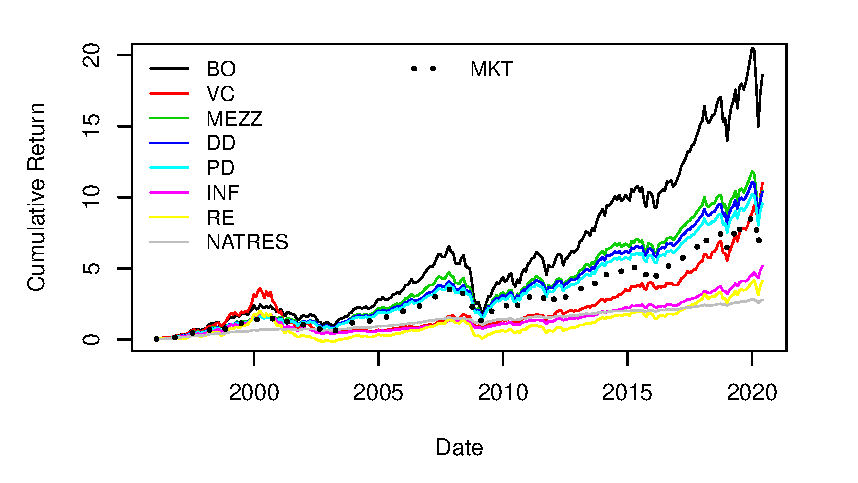
\includegraphics{Figures/Cumulative_Returns.eps}
	\caption{Cumulative USD returns implied by the MSCI World factor models from Table \ref{tab:average_coefs}.}
	\label{fig:cum_returns}   
\end{figure}


\subsection{Integrated public and private risk management}
\label{sec:integrated_risk}

In typical applications, we want to use our SDF models to analyze a blended portfolio of different private capital funds rather than investigate the factor exposure of a specific fund type.
In this case, we favor the bottom-up aggregation of SDF models to avoid overfitting.
Here, it is also straightforward to match the regional factor indices fund by fund.
In contrast, top-down selection of the 'best' SDF model for portfolio-level cash flows is likely to overfit with strongly varying SDF models for a given portfolio over time.

We consider two sets of ensembles when determining the factor exposure of actual PE portfolios.
The balanced ensemble is the set of all valid models for a given fund type (i.e., exactly the set $M^*$ as defined in subsection \ref{sec:model_averaging}).
The best ensemble is the size-$M^{**}$ subset of the balanced ensemble containing SDFs that best describes a given fund's cash flows in terms of absolute net present value error. 
Consequently, the number of components in the best ensemble is smaller than in the balanced ensemble $M^{**} \leq M^*$.
The comparison of the best and balanced model coefficients assesses how much the benchmarked portfolio's investment style differs from the average factor exposure of similar private capital portfolios.

For a sample portfolio of 100 funds visualized in figure \ref{fig:coef_barchart_100_pofo}, we see that the balanced model exhibits a MKT-RF coefficient slightly larger than one but the best SDF model MKF-RF coefficient is closer to 1.2.
This result implies higher than average market exposure for our portfolio.
Similarly, the best factor coefficients for HDY-MKT, QLT-MKT, and SMB are also higher than for the balanced ensemble.
Just the HML factor coefficient is basically the same for the best and balanced model.

Assume the asset owner of this PE portfolio is also invested in public markets.
For an integrated risk management application, the factor model derived by the best ensemble can be used as a public factor representation of the PE portfolio.
Established factor representations of any (public or private) portfolio shall be easily compatible with the asset owner's risk management framework.
Relevant methods to calculate risk measures like volatility, value-at-risk, or expected shortfall for public factor models shall be readily available in any investment risk department. 
This general approach works best if (i) the PE portfolio is diversified, and (ii) the public portfolio is still considerably larger than the PE allocation.
These conditions render an SDF model tracking error that is small in (i) absolute and (ii) relative terms and can thus be neglected.

\begin{figure}[H]
	\centering
	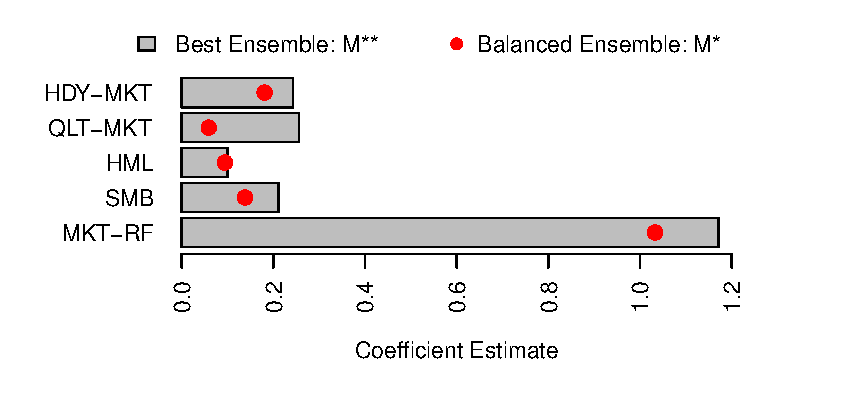
\includegraphics{Figures/Coefs100Pofo}
	\caption{Coefficient estimates of best and balanced linear SDF model for a sample portfolio consisting of 100 private capital funds.}
	\label{fig:coef_barchart_100_pofo}
\end{figure}



\section{Conclusion}
\label{sec:conclusion}

In this paper, we present a simple ensemble method to translate private equity returns to a public factor model. 
It can be used to (i) investigate public market factor exposures of private equity fund types (strategies) and to (ii) analyze actual private equity portfolios in order to enable the use of factor loadings in integrated risk management, establishing a common basis to compare the risk exposure of public and private asset portfolios. 
This novel type of analysis can complement more traditional methods of describing style and risk of private equity investments and yields additional insight for investors.
 
As a further perspective, we can amend our simple ensemble approach by more advanced ensemble learning methods like componentwise boosting \citep{B06,T19}.
Additionally, as already briefly mentioned in the article, we can apply cross-validation techniques to obtain the set of valid SDF models in a more reliable way than our simple quantile-based procedure.

%% References
\bibliographystyle{apalike}
\bibliography{ref}


\newpage


% latex table generated in R 3.6.1 by xtable 1.8-4 package
% Tue Jul 28 12:13:36 2020
\begin{table}[ht]
\centering
\begin{tabular}{lrrrrrrrr}
Vintage & BO & DD & INF & MEZZ & NATRES & PD & RE & VC \\ 
  \hline
\hline
%1983 &   0 &   0 &   0 &   0 &   0 &   0 &   0 &   0 \\ 
  1984 &   0 &   0 &   0 &   0 &   0 &   0 &   0 &   1 \\ 
  1985 &   3 &   0 &   0 &   0 &   0 &   0 &   0 &   4 \\ 
  1986 &   2 &   0 &   0 &   1 &   0 &   1 &   0 &   4 \\ 
  1987 &   4 &   0 &   0 &   1 &   0 &   1 &   0 &   3 \\ 
  1988 &   7 &   0 &   0 &   0 &   0 &   0 &   0 &   2 \\ 
  1989 &   2 &   0 &   0 &   0 &   1 &   0 &   0 &   2 \\ 
  1990 &   5 &   1 &   0 &   0 &   0 &   1 &   0 &   6 \\ 
  1991 &   3 &   2 &   0 &   0 &   0 &   2 &   0 &   4 \\ 
  1992 &   9 &   2 &   0 &   2 &   1 &   4 &   1 &   7 \\ 
  1993 &   7 &   0 &   0 &   0 &   0 &   0 &   0 &   4 \\ 
  1994 &   9 &   1 &   0 &   2 &   1 &   3 &   1 &   7 \\ 
  1995 &  17 &   0 &   0 &   1 &   1 &   1 &   1 &  10 \\ 
  1996 &  16 &   2 &   0 &   2 &   0 &   4 &   4 &  10 \\ 
  1997 &  16 &   2 &   0 &   0 &   1 &   2 &   6 &  14 \\ 
  1998 &  30 &   1 &   0 &   3 &   2 &   4 &   3 &  23 \\ 
  1999 &  28 &   1 &   0 &   7 &   1 &   8 &   2 &  37 \\ 
  2000 &  32 &   3 &   0 &   4 &   0 &   7 &   6 &  67 \\ 
  2001 &  18 &   2 &   0 &   3 &   1 &   5 &   2 &  40 \\ 
  2002 &  24 &   4 &   1 &   2 &   2 &   6 &   2 &  24 \\ 
  2003 &  18 &   3 &   1 &   2 &   1 &   5 &   6 &  19 \\ 
  2004 &  29 &   2 &   4 &   3 &   2 &   5 &  10 &  29 \\ 
  2005 &  63 &   6 &   0 &   7 &   4 &  14 &  19 &  34 \\ 
  2006 &  76 &  10 &   5 &   5 &   3 &  16 &  34 &  41 \\ 
  2007 &  88 &  13 &   5 &   3 &   7 &  16 &  36 &  53 \\ 
  2008 &  76 &  12 &   3 &   6 &   8 &  21 &  35 &  40 \\ 
  2009 &  35 &   7 &   5 &   4 &   4 &  12 &  14 &  20 \\ 
  2010 &  53 &   9 &   9 &   7 &   8 &  18 &  40 &  21 \\ 
  2011 &  72 &   8 &  11 &   6 &   9 &  16 &  51 &  27 \\ 
  2012 &  69 &  14 &   4 &  11 &  11 &  26 &  42 &  25 \\ 
  2013 &  80 &  15 &  12 &   4 &   8 &  32 &  61 &  30 \\ 
  2014 &  88 &  13 &  12 &   5 &  15 &  31 &  56 &  36 \\ 
  2015 &  99 &  18 &  13 &   7 &   9 &  38 &  86 &  47 \\ 
  2016 & 108 &   8 &  16 &   8 &  16 &  29 &  63 &  56 \\ 
  2017 &  83 &  15 &  20 &   8 &  13 &  48 &  78 &  56 \\ 
  2018 &  88 &  22 &  18 &  11 &   8 &  54 &  71 &  55 \\ 
  2019 &  21 &   3 &   5 &   2 &   1 &  11 &  12 &  11 \\ 
\hline
  Total & 1378 & 199 & 144 & 127 & 138 & 441 & 742 & 869 \\ 
   \hline
\hline
\end{tabular}
\caption{Number of funds per vintage year in the Preqin dataset used for estimation.} 
\label{tab:preqin_data}
\end{table}






\end{document}
